\begin{figure*}[!t]
\begin{tabular}{ccc}
\begin{minipage}[t]{0.23\hsize}
    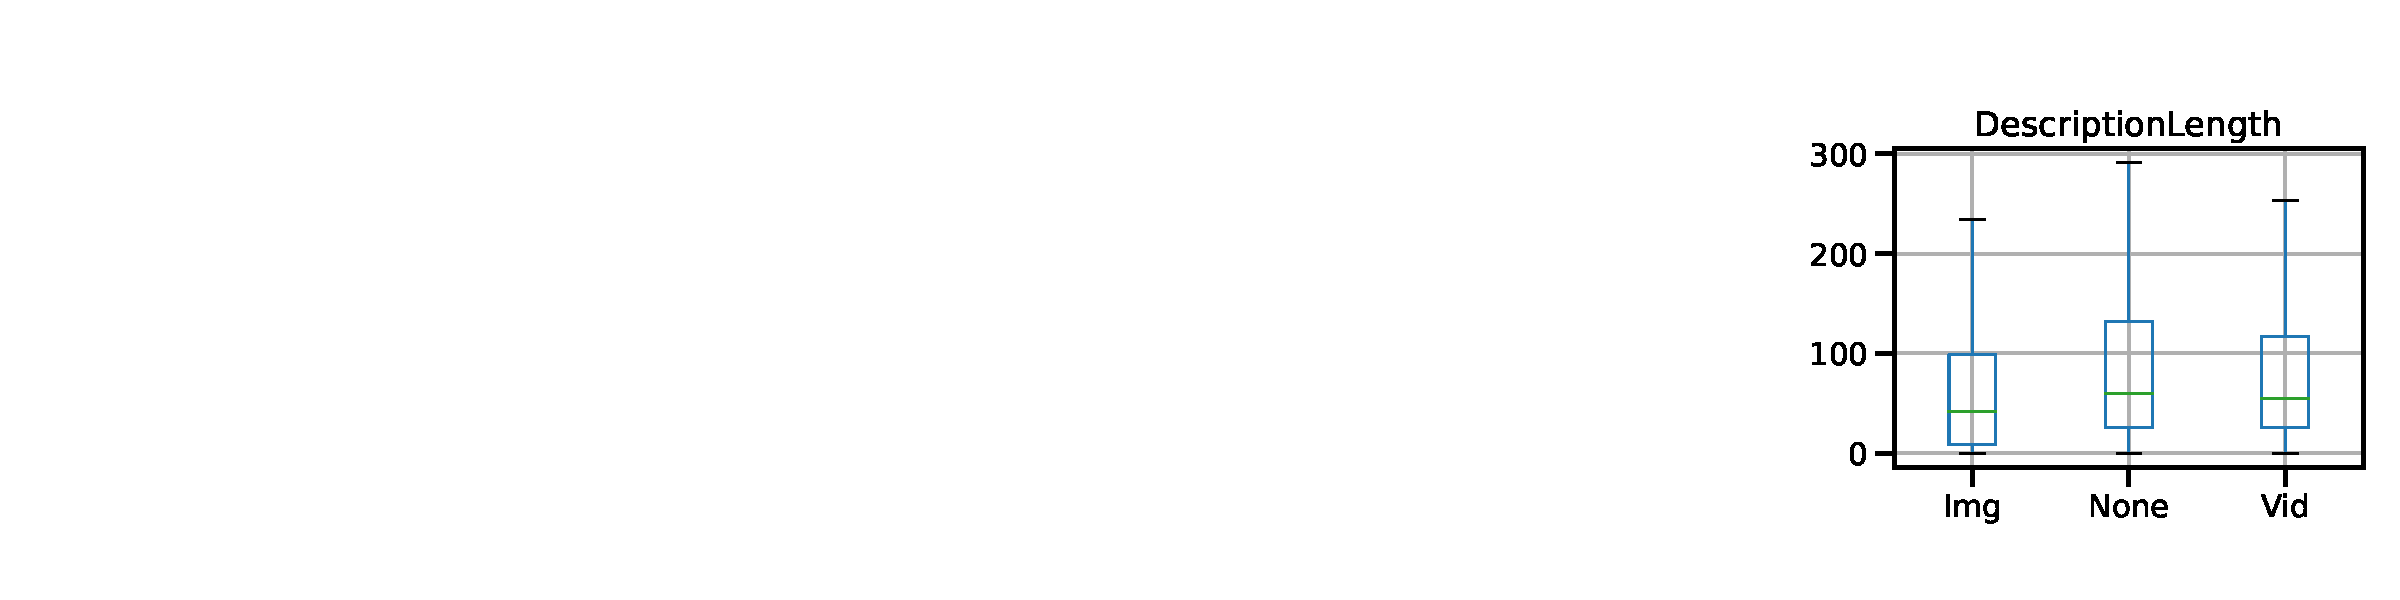
\includegraphics[width=1\linewidth]{./figures/words.pdf}
    \caption{Distribution of \#~words (``Report'' dimension)}
    \label{fig:words}
\end{minipage}
\hspace{0.04\columnwidth}
\begin{minipage}[t]{0.46\hsize}
    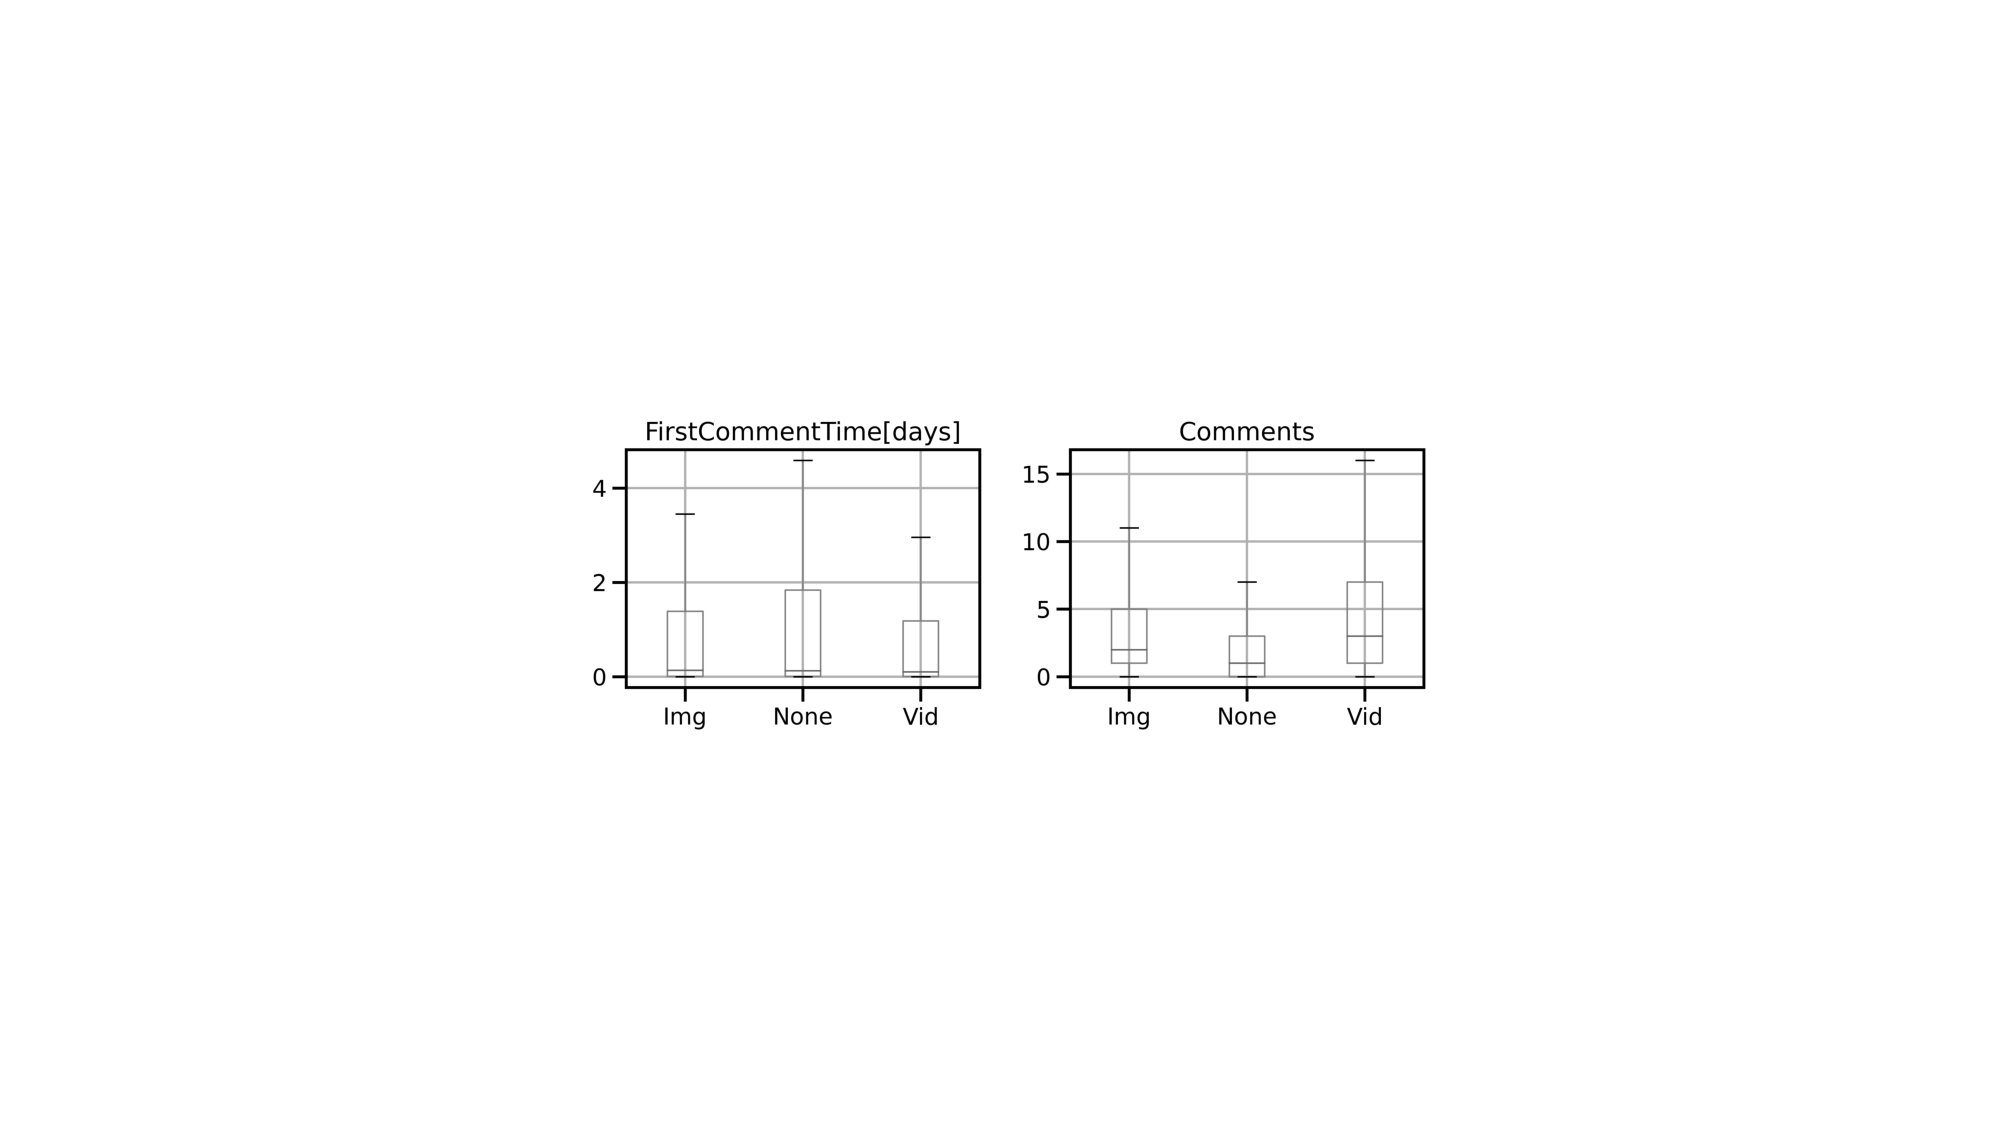
\includegraphics[width=1\linewidth]{./figures/discussions.pdf}
    %\caption{Amount of texts written in issue reports. }
    % \caption{The attributes in the Discussion dimension}
    \caption{Distribution of days to receive the first comments and the number of comments (``Discussion'' dimension)}
    \label{fig:discussion}
\end{minipage}
\hspace{0.04\columnwidth}
\begin{minipage}[t]{0.23\hsize}
    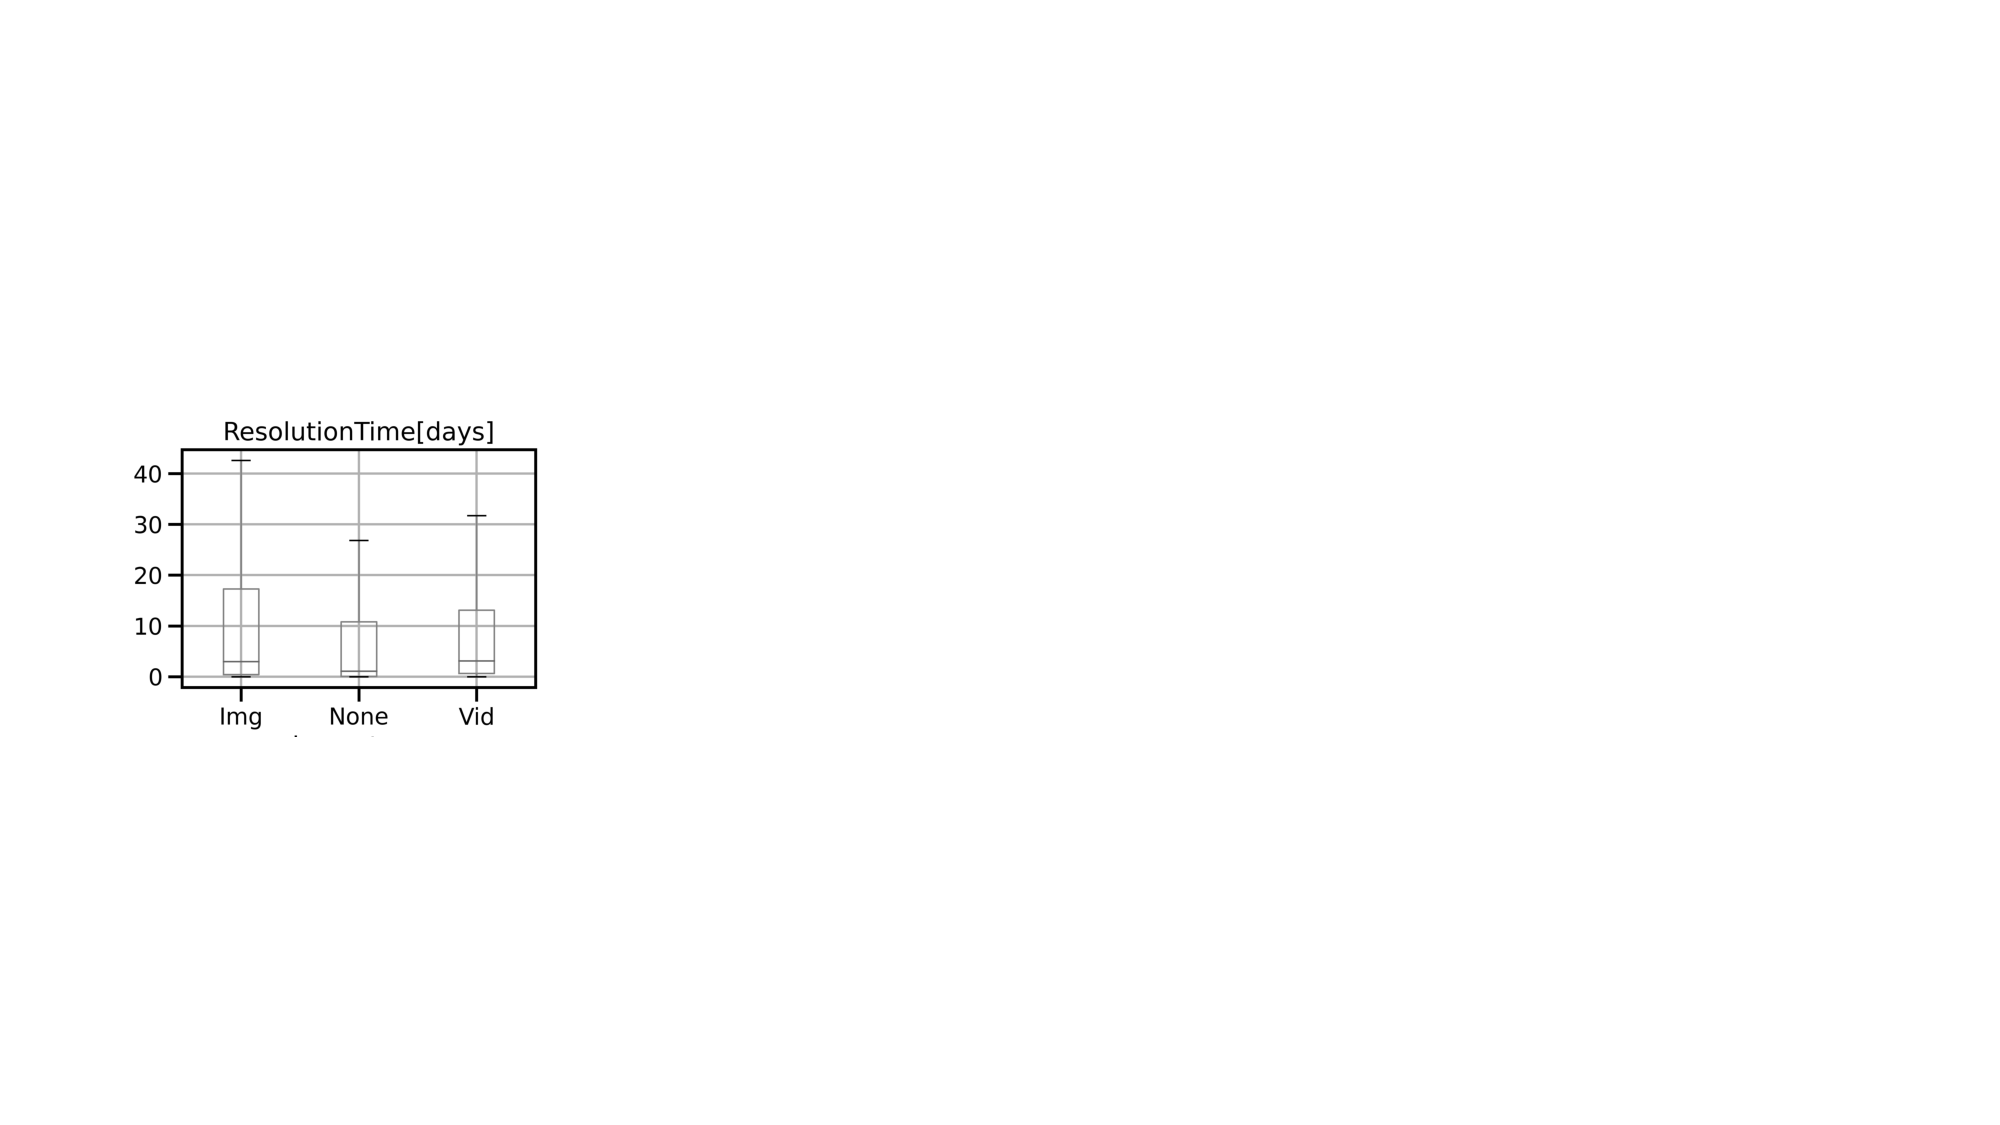
\includegraphics[width=1\linewidth]{./figures/fixes.pdf}
    \caption{Distribution of resolution time (``Fix'' dimension)}
    \label{fig:resolvedtime}
\end{minipage}
\end{tabular}
\end{figure*}



\subsection{Dataset Description}

\begin{table}[h]
    \begin{center}
    \caption{The number of issues for each category}
    \begin{tabular}{llr}
        \toprule
         & \multicolumn{1}{c}{\textbf{Description}} & \multicolumn{1}{c}{\textbf{\#issues}} \\
        \midrule
        $Img$  & $\#imgs \geq 1$ & 33,079 (4.65\%)\\
        $Mov$  & $\#movs \geq 1$ & 3,819 (0.54\%)\\
        $None$ & Others & 674,793 (94.81\%)\\ 
        \bottomrule
    \end{tabular}
    \label{classify_result}
    \end{center}
\end{table}

We classified the collected issue reports into three categories based on whether they have images and videos. 
\tab{tab:issue-category} shows the number of issue reports for each category. 
Note that issue reports often have both images and videos. 
These issue reports are counted in both $Img$ and $Vid$ categories (only around 0.05\%). 
Thus, the total number of downloaded issue reports (263,596) is different from the sum of issues (263,725).
% \#issues in \masa{Table X}\masa{Kashiwa-sensei wrote this right? I highlight the unknown table number->Yes}. 
In this paper, we refer to the issue reports in the $Img$ and $Vid$ categories
as \textit{visual issue reports}. 
\begin{figure}[h]
\centering
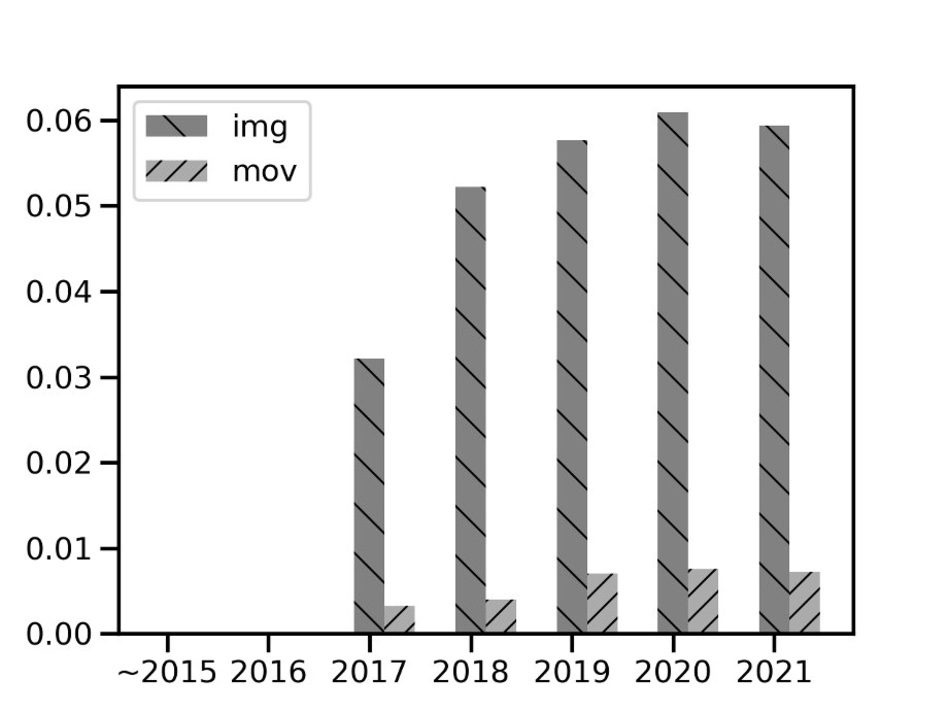
\includegraphics[width=0.6\linewidth]{./figures/data-category-trend.pdf}
\caption{ 
  The proportions of issue reports for each category
  }
\label{fig:data-cat-trend}
\end{figure}
We collected 1,324 videos and 21,003 images from 263,596 issue reports. 
Out of the collected issues, only 7.97\% of issue reports have images, and 0.50\% have videos. 
While this number seems to be small, looking into the trend shown in \fig{fig:data-cat-trend}, the rate of visual issue reports by year is increasing from 2017 to 2021. 
The ratio of visual issue reports reached to 13\% between 2017 and 2021. 
Also, we found that GitHub officially launched the function to share videos in May 2021 but developers often had uploaded videos before the beta release of the function~\citep{github-video-blog}. 
% When we looked into issue reports, GitHub had allowed users to attach GIF files on the descriptions. \kashiwa{FIXME}
When we manually looked into issue reports, GitHub had allowed users to attach GIF files on the descriptions.

\section{Results}
\label{sec:results}

% 初期段階の調査として,画像及び動画がissueの各attributesに
% 与える影響について調査する.
% 表2で得られたそれぞれのカテゴリ間で比較を比較を行う.
% 等分散性を仮定できないデータが含まれていたため,
% 比較にはSteel-Dwass testを採用する.
% 
% visualizationは,issueの解決時間,
% コメント数,文字数に何らかの影響を与える.
% 検定結果を表6に示す.
% 有意水準は0.05を採用する.
% IssueResolvedTimeにおいて,
% ImgとMovは片側検定で有意差があった.
% また,表Xより,平均値,中央値でNoneカテゴリの
% issueよりImgとMovカテゴリのissueの方が
% 課題解決時間が長かった.
% よって,画像もしくは動画がissue作成時に付与
% される課題はその解決時間が有意に長くなる.
% また,#comments及び#charsでは両側検定で
% 有意であり,これらのattributesにも
% 有意な影響を与えることがわかった.
% ただし,imageとmovieに有意差は
% 観測されなかった.

% As an initial analysis, we investigated 
% the impact of images and movies on 
% the issues in terms of the attributes. 
% As an initial analysis, 


\subsection*{RQ1: \RQone{}}
% \begin{figure}[t]
%     \centering
%     %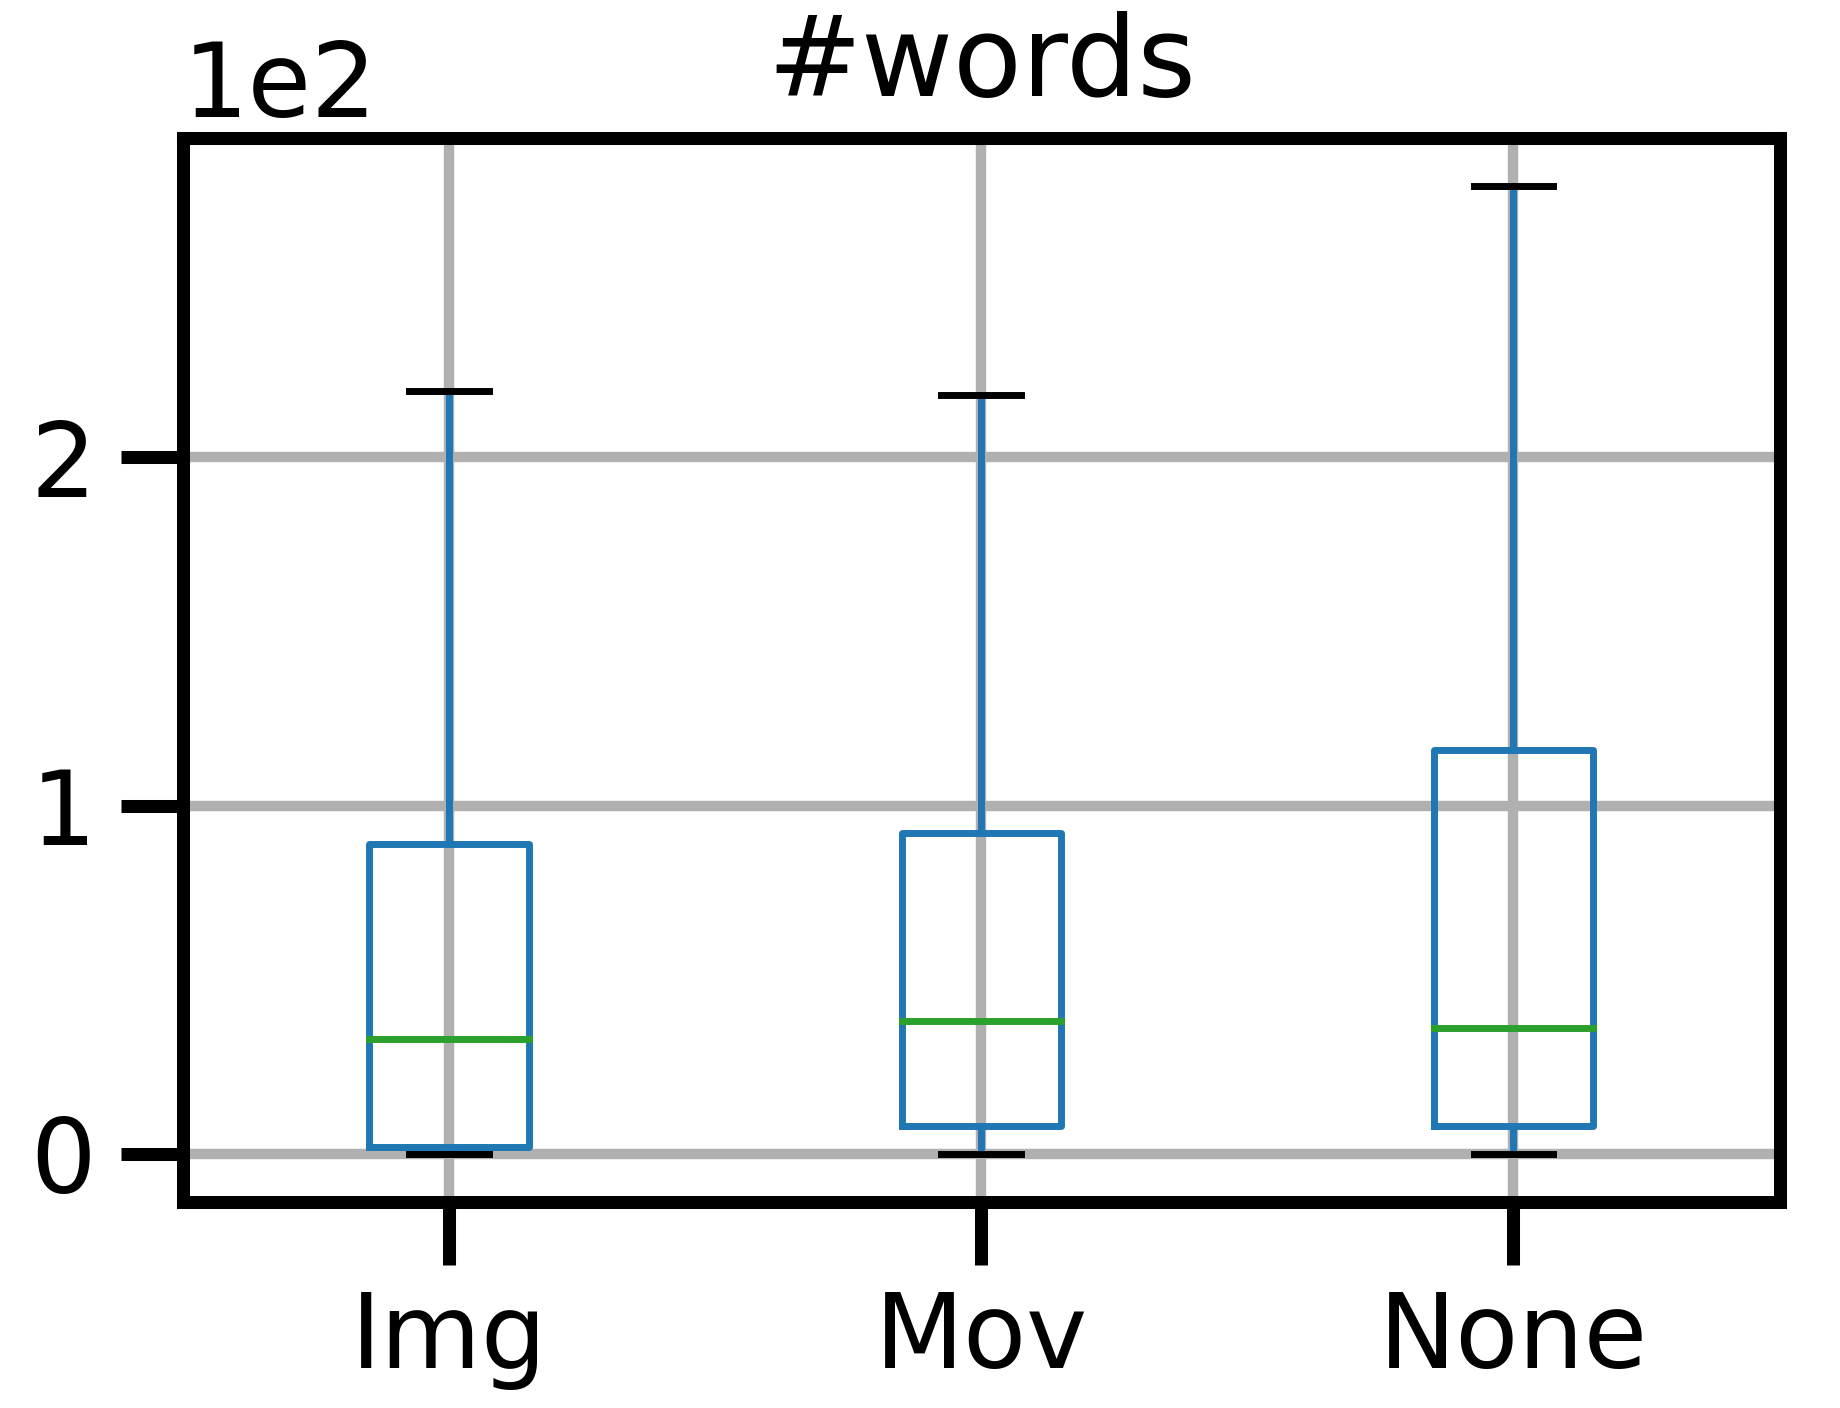
\includegraphics[width=0.5\linewidth]{tex-kondo/figures/words.png}
%     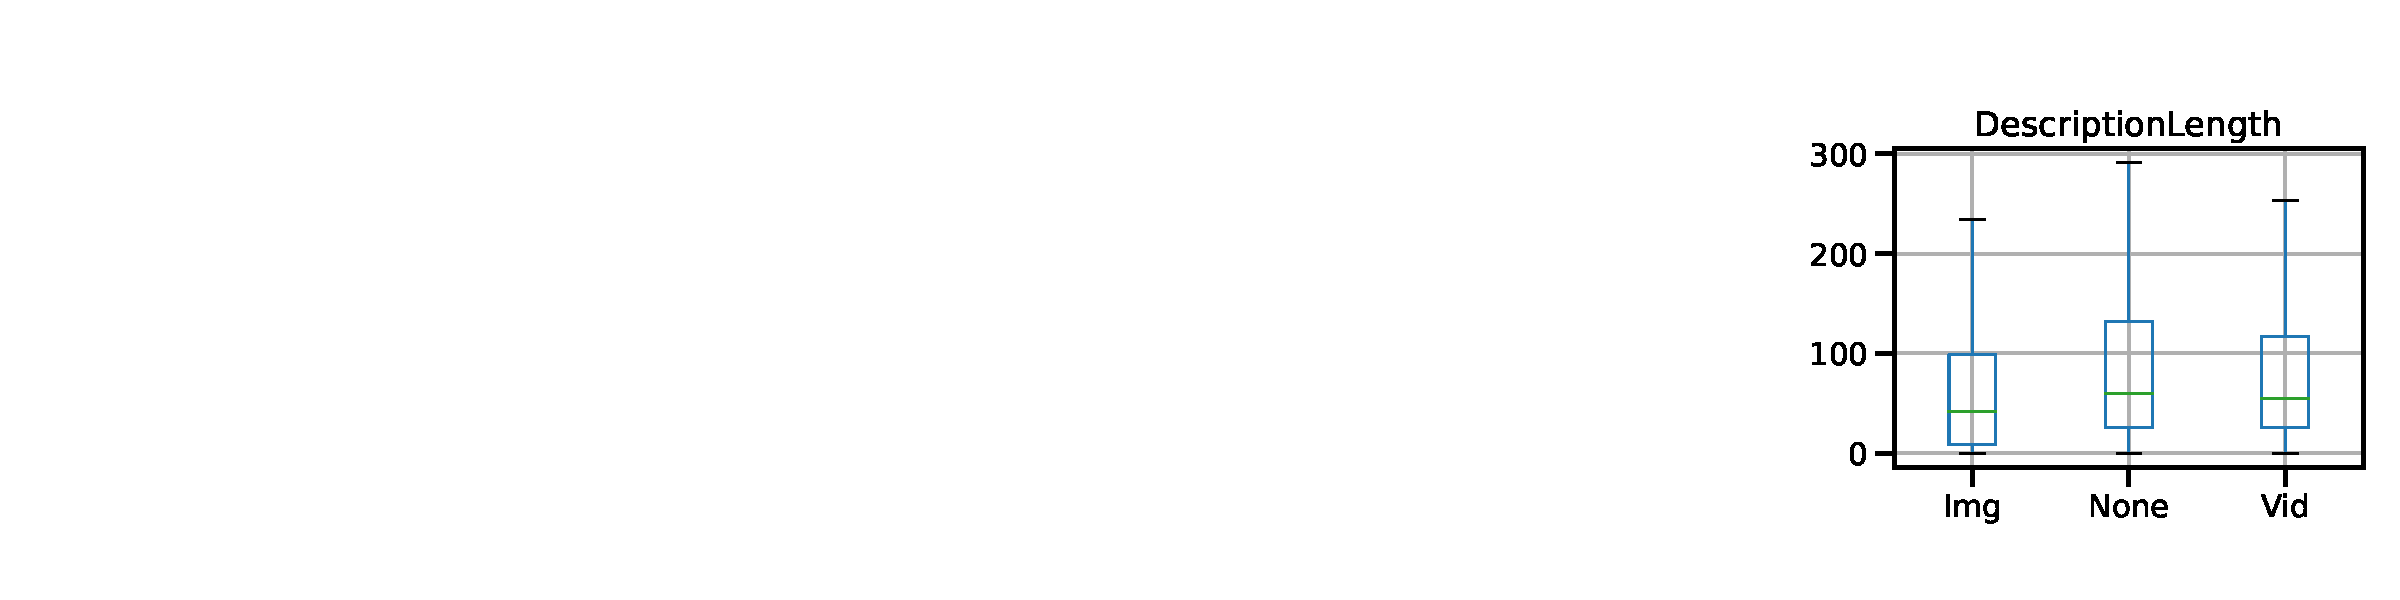
\includegraphics[width=0.5\linewidth]{./figures/words.pdf}
%     %\caption{Distributions of words written in issue reports. }
%     %\caption{Boxplots of \# of words written in the description }
%     % \caption{The attribute in the Report dimension}
%     \caption{Distribution of the number of words in the descriptions of issue reports (``Report'' dimension)}
%     \label{fig:words}
% \end{figure}
%\textbf{DescriptionLength of visual issue reports is 
%similar to the others.}

\fig{fig:words} shows the distributions in the number of words 
written in descriptions of issue reports. 
%The green line in the box shows the median, 
%the bottom and the top lines of the box show 25 and 75 percentile, respectively. 
The median of DescriptionLength was 42.0 words in Img, 
54.5 in Vid, and 60.0 in None. 
The numbers of words in the visual issue reports are slightly smaller than 
that of the non-visual ones.
% We observe statistically significant differences between the Img category and the others.
% , whereas no statistically significant differences are observed between the other combinations.
% but 
However, no statistically significant differences are observed 
between the Vid category and the None category. 
This implies that reporters write as many texts as the others 
to describe the contents of videos. 
\vspace{-0.2cm}%これは本当は入れたくないがスペースがない
\summarybox
%{Answer to RQ1}
{
% {\bf RQ1: }{No, visual issue reports still require reporters 
% to write similar amounts of texts to describe bugs. 
{\bf RQ1: }{Yes, 
% visual issue reports with images are likely to be described in fewer words, while those with videos still require reporters to write similar amounts of texts to describe bugs.
visual issue reports are likely to be described in fewer words, although no significant differences are observed between visual issue reports with videos and non-visual issue reports. 
}}

\subsection*{RQ2: \RQtwo{}}
% \begin{figure}[t]
%     \centering
%     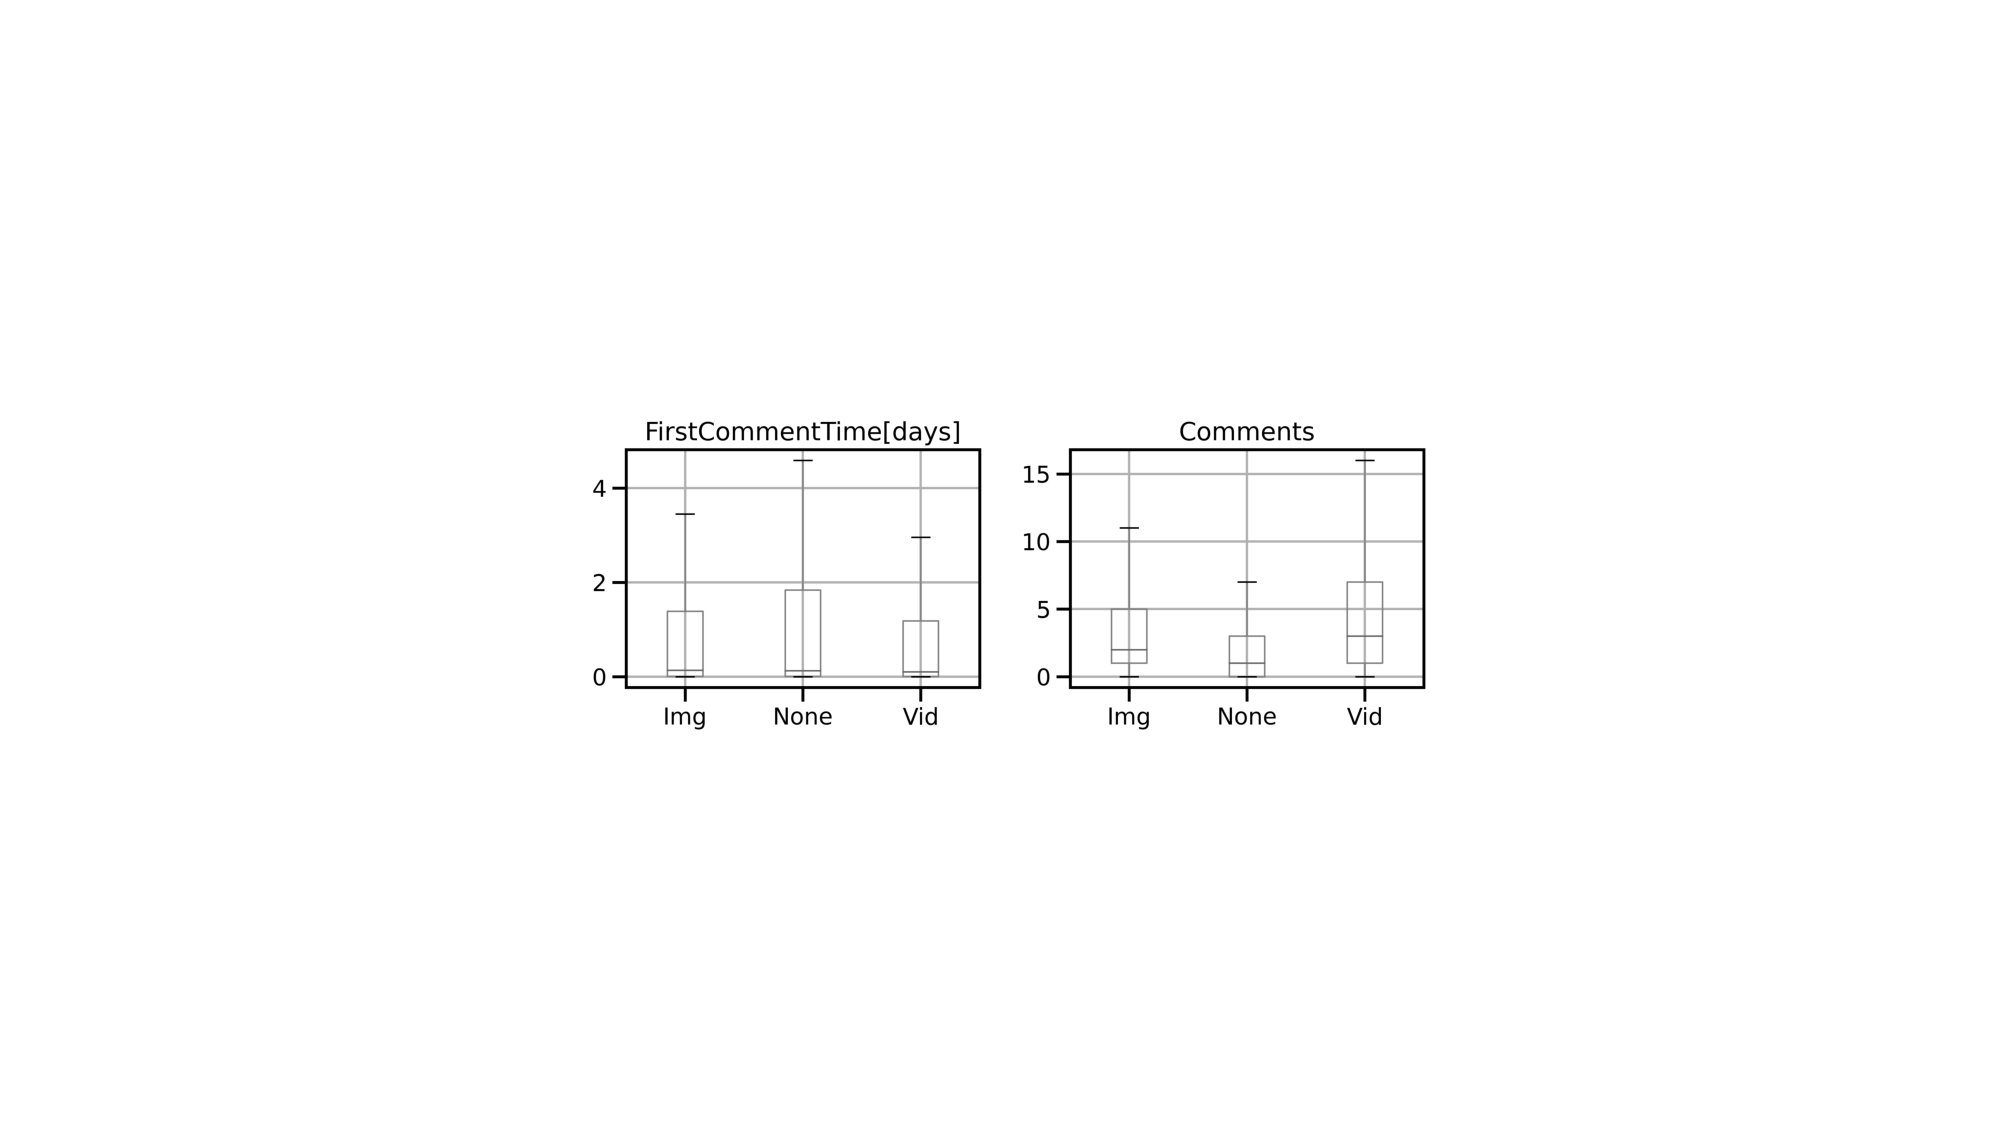
\includegraphics[width=1\linewidth]{./figures/discussions.pdf}
%     %\caption{Amount of texts written in issue reports. }
%     % \caption{The attributes in the Discussion dimension}
%     \caption{Distribution of days to receive the first comments and the number of comments (``Discussion'' dimension)}
%     \label{fig:discussion}
% \end{figure}


\fig{fig:discussion}
shows the distributions of days until the first comment made and the number of comments in issue reports. 
%% We observed that the 25th, 50th, and 75th percentiles of 
%% the $Vid$ category in 
%% this dimension
%% %$FirstCommentTime$ and $\#comments$ 
%% result in the largest or faster values than those of 
%% the other two categories.
%% Hence, the visual issue reports get more responses 
%% while they get faster responses. 
%% %% 
%% %% 
%% %% %However, we do not observe significant differences 
%% %% \textbf{
%% %% However, we occasionally observe non-significant differences
%% %% in $FirstCommentTime$ and $\#comments$.}
%% %% %\textbf{
%% %% %However, the visual issue reports are not significantly different 
%% %% %from the issue reports in the Img category
%% %% %in $FirstCommentTime$ and $\#comments$.
%% %% %}
%% %% \tab{tab:Steel-Dwass-test} shows the results of 
%% %% the Steel-Dwass test. 
%% %% 
%% %% The asterisks indicate significance based on 
%% %% the Steel-Dwass test: * indicates $p$ < 0.05 in 
%% %% the two-sided test; 
%% %% ** indicates $p$ < 0.05 in the one-sided test. 
%% %In summary, the visual issue reports do not show 
%% %significant differences compared with 
%% %the issue reports with images in 
%% %In summary, the visual issue reports are not 
%% %significantly different from the issue reports 
%% %in the Img category, 
%% %whereas visual issue reports and 
%% %the issue reports in the Img category 
%% %are significantly different from the issue reports 
%% %in the None category in
%% %$FirstCommentTime$ and $\#comments$.
%% %In summary, the visual issue reports are not 
%% However, the visual issue reports are not 
%% significantly different in $FirstCommentTime$ 
%% compared with the other two categories and 
%% are not significantly different in $Comments$ 
%% compared with the Img category.
We observed that the 25th, 50th, and 75th percentiles of the issue reports in the $Vid$ category are the longest in FirstCommentTime, whereas those of the issue reports in the $Img$ category are the shortest. 
However, no significant differences are observed. 
Also, the 25th, 50th, and 75th percentiles in Comments are the same across the categories, and no significant differences are observed. 
% Hence, the visual issue reports are not strongly related to active discussions.  
\vspace{-0.2cm}%これは本当は入れたくないがスペースがない
\summarybox
%{Summary of RQ2}
{{\bf RQ2: }{
    % Yes, visual issue reports are 3-times likely to receive more comments than reports without images or videos. 
    No, visual issue reports are not strongly related to active discussions. 
}}
\subsection*{RQ3: \RQthree{}}
% \begin{figure}[t]
%     \centering
%     %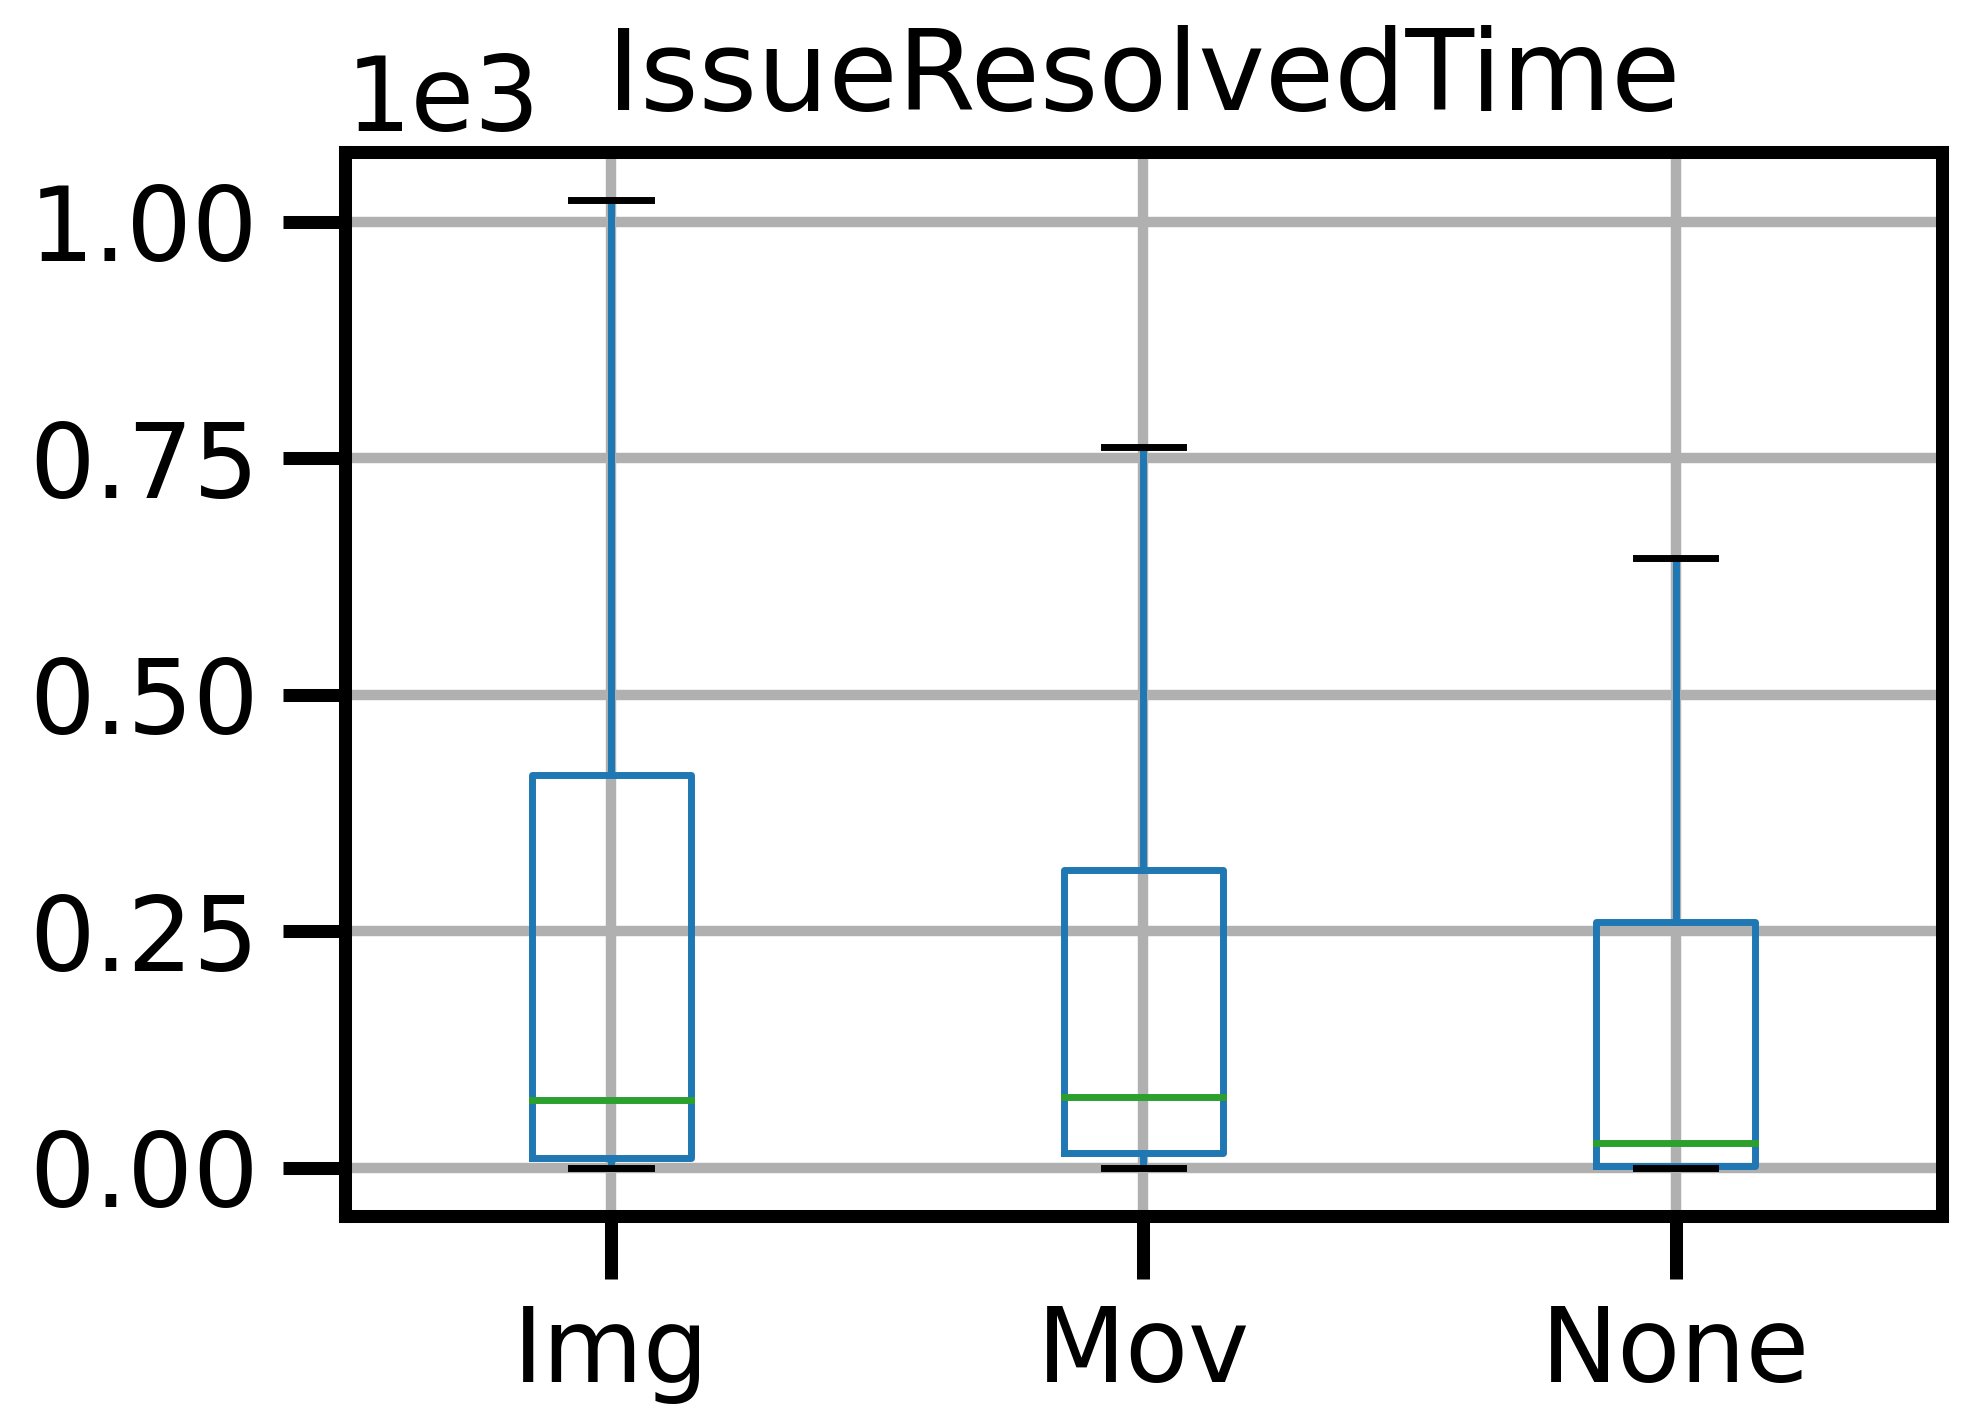
\includegraphics[width=0.6\linewidth]{tex-kondo/figures/fixes.png}
%     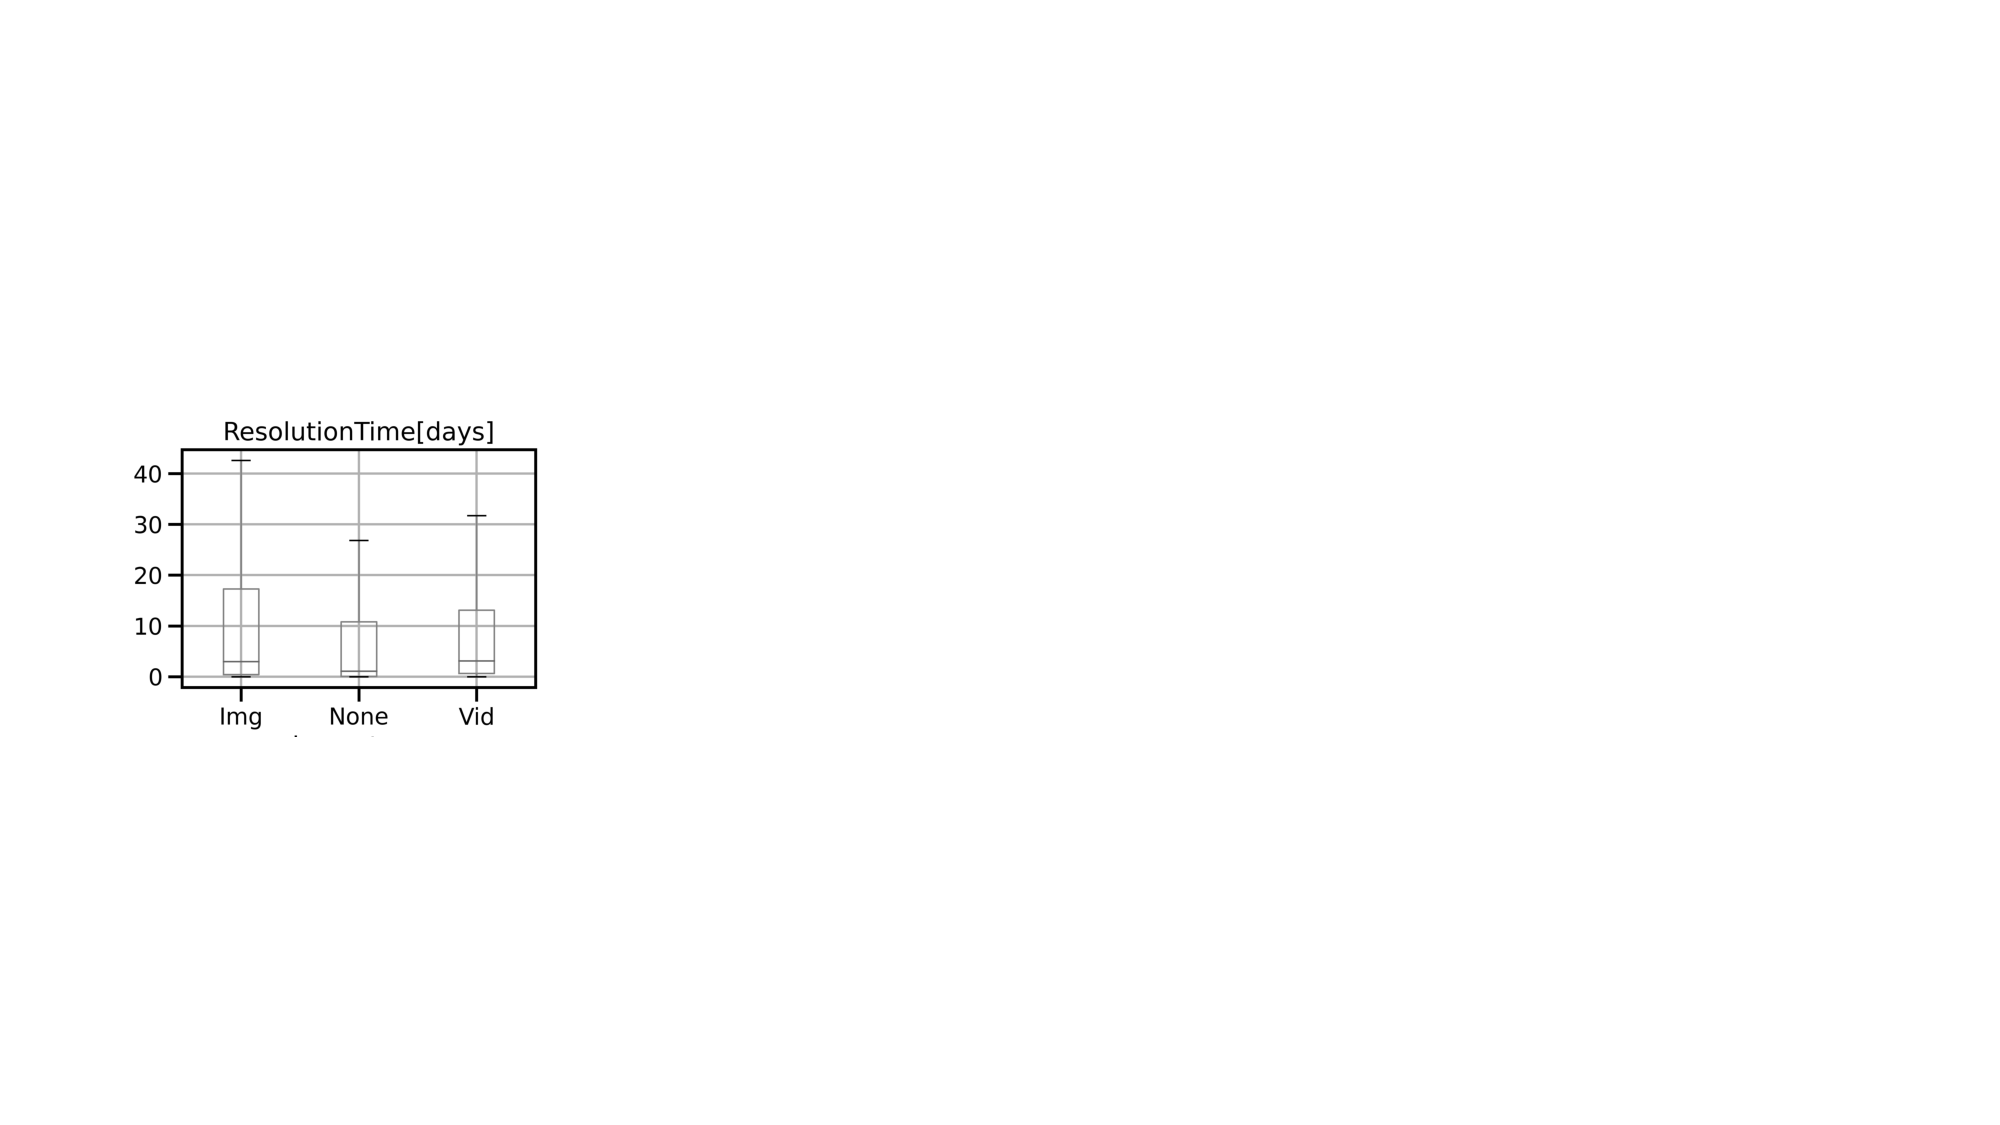
\includegraphics[width=0.5\linewidth]{./figures/fixes.pdf}
%     %\caption{Amount of texts written in issue reports. 
%     %The median of \#word was 2.96 in Img, 3.01 in Vid, and 1.09 in None.
%     %\masa{I moved this comment to here (maybe removed later? I'm not sure)}
%     %}
%     % \caption{The attribute in the Fix dimension}
%     \caption{Distribution of resolution time (``Fix'' dimension)}
%     \label{fig:resolvedtime}
% \end{figure}
%% We investigated 
%% the differences with and without images and movies 
%% for each attribute on the issues. 
%% Specifically, we compared the attributes between 
%% the categories in \tab{tab:issue-category}. 
%% Because our preliminary study shows that 
%% the distributions for each category do not 
%% come from normal distributions, 
%% we used a non-parametric test called the \textit{Steel-Dwass test}. 


%% %% %\textbf{The visual issue reports get resolved faster than 
%% %% \textbf{The visual issue reports need a longer time to be resolved than
%% %% the issue reports in the None category. }
%% %% % \textbf{The attribute values are changed 
%% % with and without images and movies.}
%% % \tab{tab:Steel-Dwass-test} shows the results of 
%% % the Steel-Dwass test. 
%% % The asterisks indicate significance based on 
%% % the Steel-Dwass test: * indicates $p$ < 0.05 in 
%% % the two-sided test; 
%% % ** indicates $p$ < 0.05 in the one-sided test. 
%% Contrary to our hypothesis, \fig{fig:resolvedtime} and our observation show that 
%% the mean and the median $ResolutionTime$ values of 
%% the issue reports in the $Img$ category and the $Vid$ category are 
%% longer than those in the $None$ category. 
%% We also observed that the issues in the $Img$ category and 
%% the $Vid$ category are significantly different from those 
%% in the $None$ category in terms of $ResolutionTime$.
%% %(\tab{tab:Steel-Dwass-test}). 
%% % \tab{tab:issue_stat_categories} shows the statistics
%% % of the collected issues for the $Img$, $Mov$,
%% % and $None$ categories.
%% % The Mean row indicates the average values; 
%% % the Min and Max rows indicate the minimum and maximum values; 
%% % the 25th, 50th, and 75th rows indicate the percentile values; 
%% % the S.D. row indicates the standard deviation values. 
%% % % We may not find the general conclusion; 
%% % % however, we observed differences across the categories. 
%% % % For example, the 25th, 50th, and 75th percentiles of 
%% % % the $Img$ and $Mov$ categories in $IssueResolvedTime$ are 
%% % % longer than those of the $None$ category. 
%% % % % \tab{tab:issue_stat_categories} shows that 
%% %This table shows that 
%% Hence, the issue reports with images or videos tend to need 
%% a longer time to be resolved. 
%% % In addition, we observed that the issues in 
%% % the $Img$ category and the $Mov$ category are 
%% % significantly different from those in 
%% % the $None$ category in terms of $\#comments$ and 
%% % $\#chars$. 
%% % Hence, the issues with images or movies 
%% % tend to have different numbers of 
%% % comments and words in the issue description.
%% % It should be noted that we do not observe 
%% % the difference between the $Img$ category and 
%% % the $Mov$ category. 
%% %{\bf No, resolution time for issues with videos are not different from those for the others. 
\fig{fig:resolvedtime} shows that the 50th and 75th percentiles of the visual issue reports are shorter than those of the non-visual issue reports in ResolutionTime.
However, the 25th percentile shows that the visual issue reports with videos need the longest resolution time. 
Also, no statistically significant differences are observed. 
\vspace{-0.2cm}%これは本当は入れたくないがスペースがない
\summarybox
%{Summary of RQ3}
{{\bf RQ3: }{
    % No, resolution time of visual issue reports is longer than that of other issue reports.
    No, resolution time of visual issue reports is not shorter/longer than that of non-visual issue reports.
}}




